\chapter{Search for H(Inv) decays in the VBF channel with CMS parked data}
\label{CHAPTER:ParkedDataAnalysis}

\glsresetall % Resetting all acronyms

This chapter describes the analysis performed over the \gls{CMS} Run I parked data collected over 2012 and 2013. This data was collected and stored without reconstruction and only became fully available a few months after data taking was finished. The advantage of this dataset is the possibility to use lower threshold triggers which can collect more signal but also more backgrounds. To take full advantage of this data the analysis had to be redesigned and extended with new control regions.

% The search for an invisible decay of a vector boson produced Higgs boson was first made public with CMS Physics Analysis Summary (PAS) HIG-13-013 which was further improved and combined with other Higgs boson production channel in the CMS paper HIG-13-30. Additional support material can be found at the CMS Analysis Notes (AN) AN-2012/403 \cite{CMS_AN_2013-403} and AN-2013/205.
% 
% During the 2012 data taking run two main streams of data were recorded. The main stream with an event rate of the order of 300 Hz to be promptly reconstructed and made available for analysis in a few days after being recorded, this dataset is referred to as the prompt data. The secondary stream with lower trigger thresholds with an event rate of the order of 1kHz which would only be reconstructed when the computing resources would be available outside of the data taking period, dataset is referred to as parked data. Our previous results
% were produced using the prompt data only and this work now extends on previous work by using the now available parked data. Since this dataset has been recorded with lower trigger thresholds the analysis was re-optimised to take advantage of this new available phase space. The details of the newly developed analysis can be found in CMS AN-14-243\cite{CMS_AN_2014-243}.
% 
%TODO: references? previous chapter?

%%%%%%%%%%%%%%%%%%%%%%%%%%%%%%%%%%%%%%%%%%%%%%%%%%%%%%%%%%%%%%%%%%%%%%%%%%%%%%%%%%%%
%%% SECTION
%%%%%%%%%%%%%%%%%%%%%%%%%%%%%%%%%%%%%%%%%%%%%%%%%%%%%%%%%%%%%%%%%%%%%%%%%%%%%%%%%%%%
\section{The Cross Check Analysis}
\label{CHAPTER:ParkedDataAnalysis_CrossCheckAnalysis}

%Status: DONE

It is normally a requirement for many CMS publications to have a cross check analysis implemented independently from the main result in order to be able to ensure accuracy of the final results due to possible errors with the software implementation. For this purpose the previous prompt data \gls{VBF} Higgs to Invisible results and publication were produced by two different and independent code frameworks and before publication a good level of synchronization was obtained. Due to lack of man power and time it was decide for the 2012-13 parked data analysis to only proceed with a single framework. At a later stage of the analysis it was thought that at least some level of cross check would be a good measure to limit the possibility of implementation errors and to allow extra confidence on the final results.
 
This cross check analysis starts from the same ntuples produced by the main analysis which were produced over all the relevant datasets. This ntuples are recorded with data formats also used by other analysis at Imperial College London, e.g. both the \gls{SM} and \gls{MSSM} Higgs to $\tau\bar{\tau}$, the Higgs to $\tau\bar{\tau}b\bar{b}$ and prompt Higgs to invisible analyses. No cuts are applied at ntuple production except the official \gls{CMS} selection for good usable data using the appropriate golden \gls{JSON} file.
 
To analyse those initial ntuple an independent code framework was developed in order to replicate all relevant numbers and plots produced by the main analysis.

%%%%%%%%%%%%%%%%%%%%%%%%%%%%%%%%%%%%%%%%%%%%%%%%%%%%%%%%%%%%%%%%%%%%%%%%%%%%%%%%%%%%
%%% SECTION
%%%%%%%%%%%%%%%%%%%%%%%%%%%%%%%%%%%%%%%%%%%%%%%%%%%%%%%%%%%%%%%%%%%%%%%%%%%%%%%%%%%%
\section{L1T Parked Trigger Development}
\label{SECTION:ParkedDataAnalysis_ParkedTriggerDevelopment}

%Status: DONE

The first step of any analysis is defining or selecting a trigger to collect data. This trigger should have a high signal efficiency while recording an acceptable rate.

At the beginning of 2012 the possibility of recording data without promptly reconstructing it was introduced. This additional data is now known as \textit{parked data}. The \gls{CMS} \gls{VBF} Higgs to invisible analysis saw this as an opportunity to develop a secondary set of triggers with lower thresholds to allow more signal to be collected when compared with the developed prompt trigger. As this effort developed it became clear that an inclusive trigger that would record \gls{VBF} events regardless of final state could be implemented.

%%%%%%%%%%%%%%%%%%%%%%%%%%%%%%%%%%%%%%%%%%%%%%%%%%%%%%%%%%%%%%%%%%%%%%%%%%%%%%%%%%%%
%%% SUBSECTION
%%%%%%%%%%%%%%%%%%%%%%%%%%%%%%%%%%%%%%%%%%%%%%%%%%%%%%%%%%%%%%%%%%%%%%%%%%%%%%%%%%%%
\subsection{VBF Higgs to Invisible Higgs Trigger}
\label{SUBSECTION:ParkedDataAnalysis_ParkedTriggerDevelopment_VBFHiggsInvisibleTrigger}

%Status: DONE

This study was based on data recorded during the high \gls{PU} special run that happened in late 2011 and was aimed at making a proposal for a viable \gls{L1T} trigger algorithm to be used during the 2012 proton run. 

The investigated algorithms select the typical topology of our signal. They look for events with \gls{MET} and and two jets located in opposite sides of the detector by requiring $\eta_{jet1}\times\eta_{jet2}<0$, large pseudo-rapidity separation of at least $\Delta\eta_{jj}>3$. The possibility of using $\Delta\phi_{jj}$ was also studied but was disfavoured since it could lead to lower signal efficiency in some \gls{BSM} models.

The conditions expected for early 2012 were of instantaneous luminosity of $5 \times 10^{33}\,\centi\meter^{-2}\second^{-1}$ and an average \gls{PU} of 28 interactions (scenario A). For late 2012 conditions were expected to increase to instantaneous luminosity of $7 \times 10^{33}\,\centi\meter^{-2}\second^{-1}$ and an average \gls{PU} of 32 interactions (scenario B).

Algorithm parameters we optimized for both this scenarios of \gls{LHC} running and considering several benchmark \gls{L1T} rates. The proposed target rate for the algorithm was assumed to be $2\,\kilo\Hz$, the additional working points were calculated with the intention to adjust the selection cuts according to higher or lower bandwidth available on the menu. The two key variables are $\pt^{\text{jets}}$ and the \gls{MET}. Each of these variables was set in turn to the lowest reasonable value while the other was scanned until the necessary rate value was achieved.  Results for scenario A can be found in table \ref{TABLE:ParkedDataAnalysis_L1TParkedTriggerDevelopment_Rate5E33} and for scenario B in table \ref{TABLE:ParkedDataAnalysis_L1TParkedTriggerDevelopment_Rate7E33}.

\begin{table}[!htb]
\begin{minipage}{.5\linewidth}
  \centering
  \begin{tabular}{|c||c|c|c|c|}
  \hline
  \multicolumn{5}{|c|}{MET [GeV] ($\pt^{\text{jets}} > 20\,\GeV$)} \\
  \hline\hline
  $\Delta\phi$ & no cut & 2.5 & 2.1 & 1.8 \\
  \hline
   $10\,\kHz$  &     32 &  32 &  32 &  32 \\
    $5\,\kHz$  &     35 &  35 &  35 &  35 \\
  \hline\hline
    $2\,\kHz$  &     41 &  41 &  41 &  41 \\
  \hline\hline
    $1\,\kHz$  &     47 &  47 &  47 &  46 \\
  $0.5\,\kHz$  &     54 &  54 &  54 &  53 \\
  \hline
  \end{tabular}
\end{minipage}%
\begin{minipage}{.5\linewidth}
  \centering
  \begin{tabular}{|c||c|c|c|c|}
  \hline
  \multicolumn{5}{|c|}{$\pt^{\text{jets}}$ [GeV] ($\text{MET}>30\,\GeV$)} \\
  \hline
  $\Delta\phi$ & no cut & 2.5 & 2.1 & 1.8 \\
  \hline\hline
   $10\,\kHz$  &     28 &  28 &  24 &  24 \\
    $5\,\kHz$  &     32 &  32 &  32 &  32 \\
  \hline\hline
    $2\,\kHz$  &     52 &  48 &  44 &  44 \\
  \hline\hline
    $1\,\kHz$  &     68 &  68 &  64 &  64 \\
  $0.5\,\kHz$  &     92 &  92 &  88 &  88 \\
  \hline
  \end{tabular}
\end{minipage} 
\caption{Tables showing the \gls{L1T} rate for different selection criteria for $5 \times 10^{33}\,\centi\meter^{-2}\second^{-1}$ and an average \gls{PU} of 28 interactions (scenario A). In selected events the leading two jets is in opposite sides of the detector. On the left table the \gls{MET} cut is calculated while requiring the two leading jets to have $\pt^{\text{jets}} > 20\,\GeV$. Similarly, on the right table $\pt^{\text{jets}}$ cut is calculated while requiring $\text{MET}>30\,\GeV$.}
\label{TABLE:ParkedDataAnalysis_L1TParkedTriggerDevelopment_Rate5E33}
\end{table}

\begin{table}[!htb]
\begin{minipage}{.5\linewidth}
  \centering
  \begin{tabular}{|c||c|c|c|c|}
  \hline
  \multicolumn{5}{|c|}{MET [GeV] ($\pt^{\text{jets}}>20\,\GeV$)} \\
  \hline\hline
  $\Delta\phi$ & no cut & 2.5 & 2.1 & 1.8 \\
  \hline
   $10\,\kHz$  &     36 &  36 &  36 &  36 \\
    $5\,\kHz$  &     40 &  40 &  40 &  40 \\
  \hline\hline
    $2\,\kHz$  &     47 &  47 &  47 &  46 \\
  \hline\hline
    $1\,\kHz$  &     54 &  54 &  54 &  54 \\
  $0.5\,\kHz$  &     67 &  66 &  66 &  64 \\
  \hline
  \end{tabular}
\end{minipage}%
  \begin{minipage}{.5\linewidth}
    \centering
  \begin{tabular}{|c||c|c|c|c|}
  \hline
  \multicolumn{5}{|c|}{$\pt^{\text{jets}}$ [GeV] ($\text{MET}>30\,\GeV$)} \\
  \hline
  $\Delta\phi$ & no cut & 2.5 & 2.1 & 1.8 \\
  \hline\hline
   $10\,\kHz$  &     32 &  32 &  32 &  32 \\
    $5\,\kHz$  &     40 &  40 &  40 &  40 \\
  \hline\hline
    $2\,\kHz$  &     64 &  60 &  60 &  56 \\
  \hline\hline
    $1\,\kHz$  &     76 &  76 &  76 &  76 \\
  $0.5\,\kHz$  &    100 & 100 &  96 &  92 \\
  \hline
  \end{tabular}
\end{minipage} 
\caption{Tables showing the \gls{L1T} rate for different selection criteria for $7 \times 10^{33}\,\centi\meter^{-2}\second^{-1}$ and an average \gls{PU} of 32 interactions (scenario B). In selected events the leading two jets is in opposite sides of the detector. On the left table the \gls{MET} cut is calculated while requiring the two leading jets to have $\pt^{\text{jets}} > 20\,\GeV$. Similarly, on the right table $\pt^{\text{jets}}$ cut is calculated while requiring $\text{MET}>30\,\GeV$.}
\label{TABLE:ParkedDataAnalysis_L1TParkedTriggerDevelopment_Rate7E33}
\end{table}

These results were used to define working points for this trigger, which were proposed to the \glsreset{TSG}
to be included on \gls{L1T} Menus. Proposed trigger options were:
\begin{itemize}
\item Algorithm A: Lead dijet (opp. sides + $\pt^{\text{jets}}>20\,\GeV$ + $\Delta\eta_{jj}>3$) + $\text{MET}>40\,\GeV$
\item Algorithm B: Lead dijet (opp. sides + $\pt^{\text{jets}}>50\,\GeV$ + $\Delta\eta_{jj}>3$) + $\text{MET}>30\,\GeV$
\end{itemize}

It can be observed that with the at the time predicted increase of luminosity the necessary rate for such proposed algorithms could escalate to $\approx 5\,\kilo\Hz$. For the rate to be maintained at $2\,\kilo\Hz$ the value of the MET cut in algorithm A would have to be raised to $47\,\GeV$ and the value of $\pt^{\text{jets}}$ cut in algorithm B would have to increase to $64\,\GeV$.

%%%%%%%%%%%%%%%%%%%%%%%%%%%%%%%%%%%%%%%%%%%%%%%%%%%%%%%%%%%%%%%%%%%%%%%%%%%%%%%%%%%%
%%% SUBSECTION
%%%%%%%%%%%%%%%%%%%%%%%%%%%%%%%%%%%%%%%%%%%%%%%%%%%%%%%%%%%%%%%%%%%%%%%%%%%%%%%%%%%%
\subsection{VBF Higgs Inclusive Trigger}
\label{SUBSECTION:ParkedDataAnalysis_ParkedTriggerDevelopment_InclusiveHiggsTrigger}

It would be desirable to have a dedicated \gls{VBF} Higgs inclusive \gls{L1T} trigger that would be decay independent. Such an algorithm would allow analysts to have a single trigger for all \gls{VBF} produced Higgs decay signatures, which would implies less systematics in their comparison. Additionally, if an algorithm is used by more analysis it will become better understood.

When selecting events based only on the presence of a dijet with \gls{VBF} characteristics we can remove the dependency on the Higgs decay. This approach would be suitable since it ignores the Higgs decays themselves. Since we are not making any assumptions of the Higgs model, we could study all possible decays even those predicted by new models with a single trigger. Thus, it would be a model-independent trigger.

This trigger can also be used for a WW scattering analysis, which in the case of the absence of the now discovered Higgs boson would allow to eventually exclude the standard model.


%%TODO: Below

For such a trigger to work it would have to be based only on the forward dijet which is the defining caracteristic
of the VBF signature.
It was decided to study two variables of the dijet system: invariant mass and transverse invariant mass (MT); and an event 
variable, scalar sum of the hadronic energy (HT). For this study we always require a dijet with $\Delta\eta>3$ and we 
look at the effects of an additional cut on $\Delta\phi$, the points tested were no cut, $<2.5$, $<2.1$ and $<1.8$.

\subsubsection{Dijet invariant mass}

This variable takes advantage from the very high invariant mass of the dijet system but it is not yet implemented
on the L1 hardware but according to trigger experts it is in principle possible to implement with the current hardware.

Unfortunately, using this variable alone to is not enough. To get acceptable rates we would need to cut too high on
jet $p_\bot$ or $M_{Inv}$ losing almost all signal efficiency.

\subsubsection{Dijet transverse invariant mass}

This variable is better at suppressing QCD events, it is less pileup-dependent and has lower error associated with it
(only x-y dependence). It is also not yet implemented on the L1 Hardware but according to trigger experts it is in principle 
possible to implement with the current hardware.

This variable showed to be promising. A possible working point for a Level 1 rate
of 5kHz could be $MT>50$ $GeV$ no $\Delta\phi$ cut and dijet $p_\bot \sim 45$ $GeV$ which should give a signal
efficiency of $\lesssim70\%$ (see R. Lane 3 Months PhD Report).

\subsubsection{Event scaler sum of the transverse energy}

Theoretically, this is the best variable to separate signal from background and has the advantage of being already
implemented on L1 hardware.

This was shown to be the most promising variable. A possible working point for a Level 1 rate of 5kHz could be $HT>100$ 
$GeV$ no $\Delta\phi$ cut and dijet $p_\bot \sim 40$ $GeV$ which should give a signal efficiency of $\lesssim98\%$
(see Figures \ref{figure_PU28_5e33_RateFBDijetDEtaDPhi00HT100} and \ref{figure_sig_eff_l1_ht}).

\begin{figure}[ht]
\centering
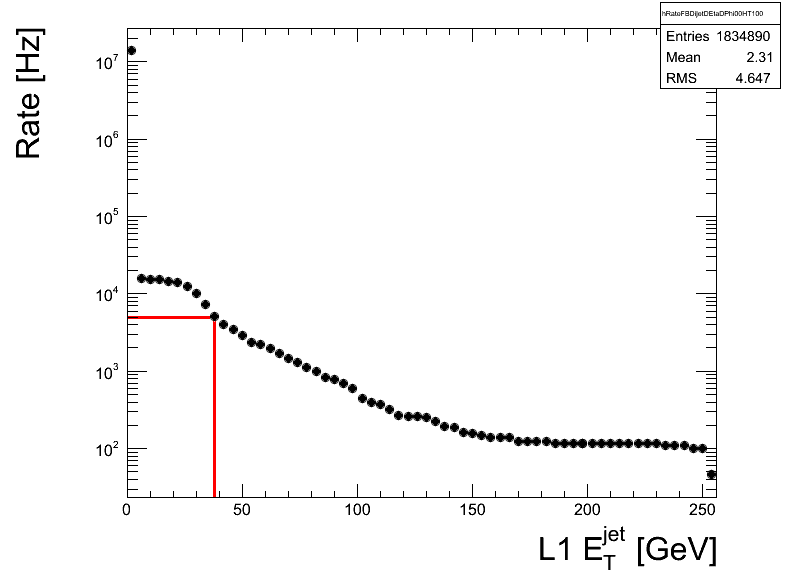
\includegraphics[width=0.60\textwidth]{Chapter06/ParkedDataTriggerDevelopment/Images/PU28_5e33_RateFBDijetDEtaDPhi00HT100.png}
\caption{Level 1 rate as a function of dijet $p_\bot$ while selecting events with $HT>100$ $GeV$. Results based on
data from the high pileup special run taken late 2011.}
\label{figure_PU28_5e33_RateFBDijetDEtaDPhi00HT100}
\end{figure}

\subsection{Final proposal}



%%%%%%%%%%%%%%%%%%%%%%%%%%%%%%%%%%%%%%%%%%%%%%%%%%%%%%%%%%%%%%%%%%%%%%%%%%%%%%%%%%%%
%%% SECTION
%%%%%%%%%%%%%%%%%%%%%%%%%%%%%%%%%%%%%%%%%%%%%%%%%%%%%%%%%%%%%%%%%%%%%%%%%%%%%%%%%%%%
\section{Data and MC samples}

%%%%%%%%%%%%%%%%%%%%%%%%%%%%%%%%%%%%%%%%%%%%%%%%%%%%%%%%%%%%%%%%%%%%%%%%%%%%%%%%%%%%
%%% SUBSECTION
%%%%%%%%%%%%%%%%%%%%%%%%%%%%%%%%%%%%%%%%%%%%%%%%%%%%%%%%%%%%%%%%%%%%%%%%%%%%%%%%%%%%
\subsection{Data}

%Status: DONE

In this analysis we used the full certified data with collisions at $\sqrt{s}=8\,\TeV$ from 2012-13 data acquisition (Run I), using golden \gls{JSON} file:

\begin{verbatim}
Cert_190456-208686_8TeV_22Jan2013ReReco_Collisions12_JSON.txt
\end{verbatim}

It amounts to an integrated luminosity of $19.2 \pm 0.5 \,\femto\barn^{-1}$. A summary of the dataset names and their integrated luminosity can be found in table \ref{TABLE:ParkedData_Data_RunI_IntegratedLuminosity}.

\begin{table}[!htb]
\centering
\begin{tabular}{|c|c|c|}
\hline
Era & Type & $\int{Luminosity}$ $[pb^{-1}]$ \\
\hline \hline
Run A & Prompt Data &  889 \\
Run B & Parked Data & 3871 \\
Run C & Parked Data & 7152 \\
Run D & Parked Data & 7317 \\
\hline\hline
\multicolumn{2}{|c|}{Total analysed} & 19229 \\
\hline\hline
\multicolumn{2}{|c|}{Total certified luminosity} & 19789 \\
\hline
\end{tabular}
\caption{Relevant parked datasets from Run I and their total analysed integrated luminosity. Total analysed and certified also showed.}
\label{TABLE:ParkedData_Data_RunI_IntegratedLuminosity}
\end{table}


The difference between certified and analysed numbers is due to our analysis trigger not being active for the first few runs of of Run 2012B.

%%%%%%%%%%%%%%%%%%%%%%%%%%%%%%%%%%%%%%%%%%%%%%%%%%%%%%%%%%%%%%%%%%%%%%%%%%%%%%%%%%%%
%%% SUBSECTION
%%%%%%%%%%%%%%%%%%%%%%%%%%%%%%%%%%%%%%%%%%%%%%%%%%%%%%%%%%%%%%%%%%%%%%%%%%%%%%%%%%%%
\subsection{Monte Carlo Samples}


%%%%%%%%%%%%%%%%%%%%%%%%%%%%%%%%%%%%%%%%%%%%%%%%%%%%%%%%%%%%%%%%%%%%%%%%%%%%%%%%%%%%
%%% SECTION
%%%%%%%%%%%%%%%%%%%%%%%%%%%%%%%%%%%%%%%%%%%%%%%%%%%%%%%%%%%%%%%%%%%%%%%%%%%%%%%%%%%%
\section{Monte Carlo to Data correction factors}

%Status: DONE

To correctly compare \gls{MC} with data all relevant aspects must be correctly taken into account. In the event that a variable distribution does not match between both we can determine weights to apply to each event so the distributions match again. In these analysis we apply four weights to \gls{MC}, to obtain the correct \gls{PU} distribution, weight events according to the probability of passing the trigger, account for lepton identification probability and top sample re-weghting.

%%%%%%%%%%%%%%%%%%%%%%%%%%%%%%%%%%%%%%%%%%%%%%%%%%%%%%%%%%%%%%%%%%%%%%%%%%%%%%%%%%%%
%%% SUBSECTION
%%%%%%%%%%%%%%%%%%%%%%%%%%%%%%%%%%%%%%%%%%%%%%%%%%%%%%%%%%%%%%%%%%%%%%%%%%%%%%%%%%%%
\subsection{Pile-up}

%%%%%%%%%%%%%%%%%%%%%%%%%%%%%%%%%%%%%%%%%%%%%%%%%%%%%%%%%%%%%%%%%%%%%%%%%%%%%%%%%%%%
%%% SUBSECTION
%%%%%%%%%%%%%%%%%%%%%%%%%%%%%%%%%%%%%%%%%%%%%%%%%%%%%%%%%%%%%%%%%%%%%%%%%%%%%%%%%%%%
\subsection{Trigger efficiency}
\label{SUBSECTION:ParkedDataAnalysis_CorrectionFactors_TriggerEfficiency}

%Status: DONE

The initial event selection for this analysis starts with a dedicated set of triggers which were recorded to the \gls{VBF} parked dataset. We used the following \gls{HLT} trigger paths for each Run I era:

\begin{itemize}
  \item Run A:       \verb!HLT_DiPFJet40_PFMETnoMu65_MJJ800VBF_AllJets!
  \item Run B and C: \verb!HLT_DiJet35_MJJ700_AllJets_DEta3p5_VBF!
  \item Run D:       \verb!HLT_DiJet30_MJJ700_AllJets_DEta3p5!
\end{itemize}

All the used paths are seeded by \gls{L1T} trigger condition \verb!L1_ETM40!. 


To maximize the usage of the event statistics of the selected \gls{MC} samples, we do not veto events that fail the trigger conditions. Instead an event by event weight is calculated which which taking into account how much luminosity was recorded by each of the three trigger and depending on the offline quantities which correspond to the ones used in the trigger conditions: PFMETnoMu, leading dijet $m_{jj}$ and sub-leading jet \pt. 

To define the weights, turn on curves were determined according to these offline variables as a function of PFMETnoMu in bins of dijet $m_{jj}$ and sub-leading jet \pt. This approach allows the determination of the weights which include the correlations between these variables. The turn on curves are obtained by fitting equation \ref{EQUATION:ParkedDataAnalysis_TriggerEfficiency_Efficiency} to each bin.

\begin{equation}
\frac{\varepsilon_{max}}{2}\text{Erf}\left(\frac{x-x_{0}}{\sqrt{\Gamma}}\right)+1,
\label{EQUATION:ParkedDataAnalysis_TriggerEfficiency_Efficiency} 
\end{equation}

Where $\varepsilon_{max}$ os the maximum efficiency of the trigger in the bin, $x_{0}$ is the mid-value of the turn on and $\Gamma$ is the width of the turn on.

%%%%%%%%%%%%%%%%%%%%%%%%%%%%%%%%%%%%%%%%%%%%%%%%%%%%%%%%%%%%%%%%%%%%%%%%%%%%%%%%%%%%
%%% SUBSECTION
%%%%%%%%%%%%%%%%%%%%%%%%%%%%%%%%%%%%%%%%%%%%%%%%%%%%%%%%%%%%%%%%%%%%%%%%%%%%%%%%%%%%
\subsection{Lepton Identification}

%%%%%%%%%%%%%%%%%%%%%%%%%%%%%%%%%%%%%%%%%%%%%%%%%%%%%%%%%%%%%%%%%%%%%%%%%%%%%%%%%%%%
%%% SUBSECTION
%%%%%%%%%%%%%%%%%%%%%%%%%%%%%%%%%%%%%%%%%%%%%%%%%%%%%%%%%%%%%%%%%%%%%%%%%%%%%%%%%%%%
\subsection{Top reweighting}

%%%%%%%%%%%%%%%%%%%%%%%%%%%%%%%%%%%%%%%%%%%%%%%%%%%%%%%%%%%%%%%%%%%%%%%%%%%%%%%%%%%%
%%% SECTION
%%%%%%%%%%%%%%%%%%%%%%%%%%%%%%%%%%%%%%%%%%%%%%%%%%%%%%%%%%%%%%%%%%%%%%%%%%%%%%%%%%%%
\section{Signal event selection}

%%%%%%%%%%%%%%%%%%%%%%%%%%%%%%%%%%%%%%%%%%%%%%%%%%%%%%%%%%%%%%%%%%%%%%%%%%%%%%%%%%%%
%%% SECTION
%%%%%%%%%%%%%%%%%%%%%%%%%%%%%%%%%%%%%%%%%%%%%%%%%%%%%%%%%%%%%%%%%%%%%%%%%%%%%%%%%%%%
\section{Control Regions}

%%%%%%%%%%%%%%%%%%%%%%%%%%%%%%%%%%%%%%%%%%%%%%%%%%%%%%%%%%%%%%%%%%%%%%%%%%%%%%%%%%%%
%%% SUBSECTION
%%%%%%%%%%%%%%%%%%%%%%%%%%%%%%%%%%%%%%%%%%%%%%%%%%%%%%%%%%%%%%%%%%%%%%%%%%%%%%%%%%%%
\subsection{Top background estimation}

%%%%%%%%%%%%%%%%%%%%%%%%%%%%%%%%%%%%%%%%%%%%%%%%%%%%%%%%%%%%%%%%%%%%%%%%%%%%%%%%%%%%
%%% SUBSECTION
%%%%%%%%%%%%%%%%%%%%%%%%%%%%%%%%%%%%%%%%%%%%%%%%%%%%%%%%%%%%%%%%%%%%%%%%%%%%%%%%%%%%
\subsection{W background estimation}

%%%%%%%%%%%%%%%%%%%%%%%%%%%%%%%%%%%%%%%%%%%%%%%%%%%%%%%%%%%%%%%%%%%%%%%%%%%%%%%%%%%%
%%% SUBSECTION
%%%%%%%%%%%%%%%%%%%%%%%%%%%%%%%%%%%%%%%%%%%%%%%%%%%%%%%%%%%%%%%%%%%%%%%%%%%%%%%%%%%%
\subsection{W background estimation}

%%%%%%%%%%%%%%%%%%%%%%%%%%%%%%%%%%%%%%%%%%%%%%%%%%%%%%%%%%%%%%%%%%%%%%%%%%%%%%%%%%%%
%%% SUBSUBSECTION
%%%%%%%%%%%%%%%%%%%%%%%%%%%%%%%%%%%%%%%%%%%%%%%%%%%%%%%%%%%%%%%%%%%%%%%%%%%%%%%%%%%%
\subsubsection{W to electron+neutrino}

%%%%%%%%%%%%%%%%%%%%%%%%%%%%%%%%%%%%%%%%%%%%%%%%%%%%%%%%%%%%%%%%%%%%%%%%%%%%%%%%%%%%
%%% SUBSUBSECTION
%%%%%%%%%%%%%%%%%%%%%%%%%%%%%%%%%%%%%%%%%%%%%%%%%%%%%%%%%%%%%%%%%%%%%%%%%%%%%%%%%%%%
\subsubsection{W to muon+neutrino}

%%%%%%%%%%%%%%%%%%%%%%%%%%%%%%%%%%%%%%%%%%%%%%%%%%%%%%%%%%%%%%%%%%%%%%%%%%%%%%%%%%%%
%%% SUBSUBSECTION
%%%%%%%%%%%%%%%%%%%%%%%%%%%%%%%%%%%%%%%%%%%%%%%%%%%%%%%%%%%%%%%%%%%%%%%%%%%%%%%%%%%%
\subsubsection{W to tau+neutrino}

%%%%%%%%%%%%%%%%%%%%%%%%%%%%%%%%%%%%%%%%%%%%%%%%%%%%%%%%%%%%%%%%%%%%%%%%%%%%%%%%%%%%
%%% SUBSECTION
%%%%%%%%%%%%%%%%%%%%%%%%%%%%%%%%%%%%%%%%%%%%%%%%%%%%%%%%%%%%%%%%%%%%%%%%%%%%%%%%%%%%
\subsection{Z background estimation}

%%%%%%%%%%%%%%%%%%%%%%%%%%%%%%%%%%%%%%%%%%%%%%%%%%%%%%%%%%%%%%%%%%%%%%%%%%%%%%%%%%%%
%%% SUBSECTION
%%%%%%%%%%%%%%%%%%%%%%%%%%%%%%%%%%%%%%%%%%%%%%%%%%%%%%%%%%%%%%%%%%%%%%%%%%%%%%%%%%%%
\subsection{QCD background estimation}

%%%%%%%%%%%%%%%%%%%%%%%%%%%%%%%%%%%%%%%%%%%%%%%%%%%%%%%%%%%%%%%%%%%%%%%%%%%%%%%%%%%%
%%% SUBSUBSECTION
%%%%%%%%%%%%%%%%%%%%%%%%%%%%%%%%%%%%%%%%%%%%%%%%%%%%%%%%%%%%%%%%%%%%%%%%%%%%%%%%%%%%
\subsubsection{QDC VBF-like + MET Monte Carlo Sample}

%%%%%%%%%%%%%%%%%%%%%%%%%%%%%%%%%%%%%%%%%%%%%%%%%%%%%%%%%%%%%%%%%%%%%%%%%%%%%%%%%%%%
%%% SUBSUBSECTION
%%%%%%%%%%%%%%%%%%%%%%%%%%%%%%%%%%%%%%%%%%%%%%%%%%%%%%%%%%%%%%%%%%%%%%%%%%%%%%%%%%%%
\subsubsection{Data driven QCD estimation}

%%%%%%%%%%%%%%%%%%%%%%%%%%%%%%%%%%%%%%%%%%%%%%%%%%%%%%%%%%%%%%%%%%%%%%%%%%%%%%%%%%%%
%%% SECTION
%%%%%%%%%%%%%%%%%%%%%%%%%%%%%%%%%%%%%%%%%%%%%%%%%%%%%%%%%%%%%%%%%%%%%%%%%%%%%%%%%%%%
\section{Systematics}

%%%%%%%%%%%%%%%%%%%%%%%%%%%%%%%%%%%%%%%%%%%%%%%%%%%%%%%%%%%%%%%%%%%%%%%%%%%%%%%%%%%%
%%% SECTION
%%%%%%%%%%%%%%%%%%%%%%%%%%%%%%%%%%%%%%%%%%%%%%%%%%%%%%%%%%%%%%%%%%%%%%%%%%%%%%%%%%%%
\section{Results}

%%%%%%%%%%%%%%%%%%%%%%%%%%%%%%%%%%%%%%%%%%%%%%%%%%%%%%%%%%%%%%%%%%%%%%%%%%%%%%%%%%%%
%%% SECTION
%%%%%%%%%%%%%%%%%%%%%%%%%%%%%%%%%%%%%%%%%%%%%%%%%%%%%%%%%%%%%%%%%%%%%%%%%%%%%%%%%%%%
\section{Extraction of limits}

% %%%%%%%%%%%%%%%%%%%%%%%%%%%%%%%%%%%%%%%%%%%%%%%%%%%%%%%%%%%%%%%%%%%%%%%%%%%%%%%%%%%%
% %%% SECTION
% %%%%%%%%%%%%%%%%%%%%%%%%%%%%%%%%%%%%%%%%%%%%%%%%%%%%%%%%%%%%%%%%%%%%%%%%%%%%%%%%%%%%
% \section{Event quality filters}
% 
% During data recording issues may happen with the detector or data acquisition which may render some of the events unusable. The groups responsible for each part of the detector and physics object check the data after it was taken and if they find such problems occurred. This groups produce software event filters analysts to be able to remove this problematic events. This issues cover from know detector problems to miss firing of calibration sequences or even failure to reconstruct physics objects.
% 
% The Jet-MET Particle Object Group (POG) recommends the usage of the following filters which are used in this analysis.
% % \cite{CMS:JetMETPOG:MissingETOptionalFilters}
% 
% \begin{itemize}
%   \item CSCTightHaloFilter
%   \item HBHENoiseFilter
%   \item EcalDeadCellTriggerPrimitiveFilter
%   \item trackingFailureFilter
%   \item eeBadScFilter
%   \item ECAL Laser filter
%   \item HCAL Laser filter
% \end{itemize}
% 
% In turn the JetMET group recommend the usage of the following Tracking POG Filter:
% %\cite{CMS:TrackingPOG:TrackingPOGFilters}
% 
% 
% \begin{itemize}
%   \item logErrorTooManyClusters
%   \item manystripclus53X
%   \item toomanystripclus53X
% \end{itemize}
